%!TEX root = ../report.tex

\section{Experiments}

\subsection{Simulated examples}
In this part, we reproduce and extend the section "Simulated Scenarios" by writing our own python codes from scratch based on the Matlab version of the original paper \cite{simu_code}. A number of simulated experiments are conducted to validate theoretical results and demonstrate the differences between (1) standard HMC, (2) the naive implementation of stochastic gradient HMC, which simply replaces the gradient with a stochastic gradient, and (3) the proposed method incorporating friction, SGHMC. We also compare SGHMC to the first-order Langevin dynamics of SGLD.

Firstly, to explore the performances of various sampling methods with exact gradients relative to stochastic gradients, we set up several simulated experiments based on the the true target distribution with $U(\theta) = -2\theta^2 + \theta^4$ mentioned in original paper. Also, we test on $U(\theta) = \frac{1}{2}\theta^2$ as a simple extension which can help us confirm the conclusion here and also help us more thoroughly understand the Fig. 2(a) that has the same target distribution. 

\begin{figure}[h!]
\begin{subfigure}{.5\textwidth}
\includegraphics[width=.9\linewidth]{parts/Images/fig1a.pdf}
\caption{Distributions of different sampling algorithms for the target function $U(\theta) = -2\theta^2 + \theta^4$}
\label{fig1a}
\end{subfigure}%
\begin{subfigure}{.5\textwidth}
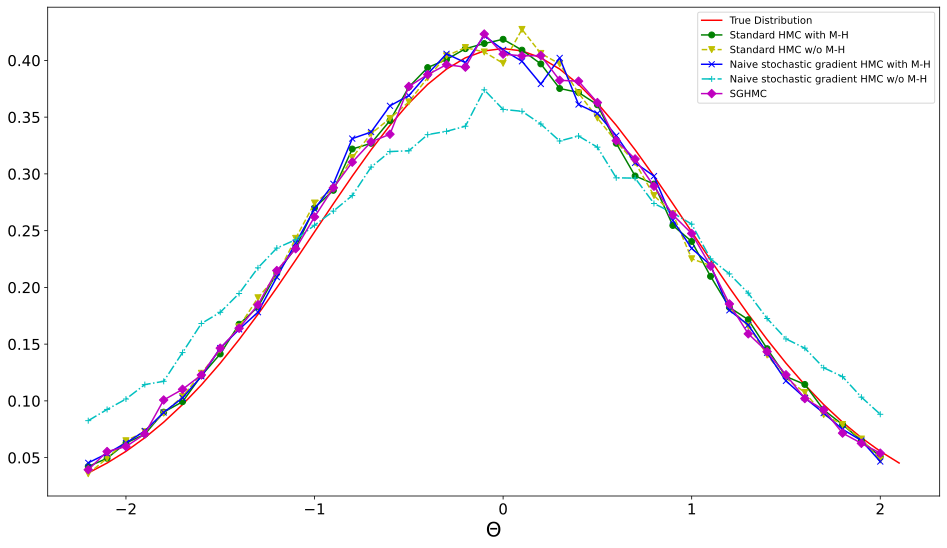
\includegraphics[width=.9\linewidth]{parts/Images/fig1b.pdf}
\caption{Distributions of different sampling algorithms for the target function $U(\theta) = \frac{1}{2}\theta^2$}
\label{fig1b}
\end{subfigure}
\caption{Empirical distributions associated with various sampling algorithms relative to the different true target distributions.}
\label{fig:demo}
\end{figure}

As a baseline, we consider the standard HMC methods, both with and without the MH correction. Then we compare with the naive stochastic HMC methods in Alg. 1 of Section 2.1, which simply replaces $\nabla U(\theta)$ with $\nabla \wt{U}(\theta)$, both with and without as MH correction same as the above. Finally, we compare to the SGHMC, Alg. 2 of Section 2.3, without MH correction. Specifically, based on the current model parameters and sample size, 4 is chosen as the covariance of the stochastic gradient noise. Hence, $\nabla \wt{U}(\theta) = \nabla U(\theta) + \mathcal{N}(0,4)$ is used for stochastic gradient based samplers. And $\epsilon = 0.1$  is employed for all the cases. In all variants of HMC above, the momentum is resampled every 50 steps.

Compared with results in Fig. 1 of the original paper, we perfectly reproduce the simulations on the true distribution $U(\theta) = -2\theta^2 + \theta^4$ in Fig. 1(a). Also, we produce the tests on another true distribution $U(\theta) = \frac{1}{2}\theta^2$ as shown in Fig. 1(b). From both figures, we can see that both the HMC and SGHMC algorithms match perfectly with the target function even without an MH correction, which validates the theoretical results; that is, both standard HMC and SGHMC maintain $\pi$ as the invariant distribution as $\epsilon \rightarrow 0$. However, the natural implementation of the stochastic approximation can be arbitrarily bad without MH step. This can be explained by the Corollary 3.1 in original paper. Because $\pi$ is no longer invariant under the dynamics of naive stochastic gradient HMC, a correction step must be introduced even before considering errors introduced by the discretization of the dynamical system in practice.

As a conclusion, HMC with stochastic gradients requires a frequent costly MH correction step since the noise injected by the stochastic gradient no longer leads to Hamiltonian dynamics with the desired stationary target distribution. In contrary, SGHMC introduces a variant that uses second-order Langevin dynamics with a friction term that counteracts the effects of the noisy gradient, maintaining the desired target distribution as the invariant distribution.

Secondly, to simply simulating from the discretized Hamiltonian dynamical systems with the various samplers compared, we compare their resulting trajectories of points $(\theta,r)$.  The compared methods are totally the same as the above. As for the details, discretization of various HMC methods are implemented in 15000 steps using the target distribution $U(\theta) = \frac{1}{2}\theta^2$ and $\epsilon$ is set as 0.1. For the noisy scenarios, the gradient is replaced by $\nabla \wt{U}(\theta) = \nabla U(\theta) + \mathcal{N}(0,4)$, the same as Fig. 1(b).

\begin{figure}[h!]
    \centering
    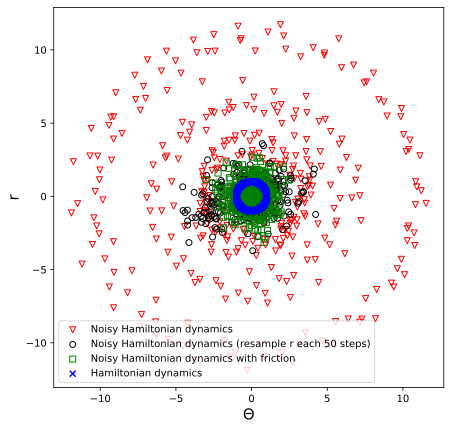
\includegraphics[width=0.6\linewidth]{parts/Images/fig2a.pdf}%
    \caption{Step equals to 15000}
     \label{fig:a}%
\end{figure}

Compared with results in Fig. 2 of the original paper, we reproduce the Fig. 2(a) in a perfect way. And we find that the path of $(\theta,r)$ from the noisy Hamiltonian system without any friction or steps diverges significantly. To correct the divergence, the naive stochastic gradient HMC without MH steps can be implemented through periodic resampling of the momentum, which may not yield the correct target distribution, as illustrated in Fig. 1(b). Then to correct this behaviour, SGHMC can be used to modify this dynamical system. The results can show that the straightforward modification to the Hamiltonian dynamics can alleviate the issues of the noise introduced by stochastic gradients. In particular, the modification allows us to again achieve the desired $\pi$ as the invariant distribution of the continuous Hamiltonian dynamical system. Moreover, Fig. 2(a) can help explain Corollary 3.1 in the original paper by seeing that even finite-length simulations from the noisy system can diverge quite substantially from those of the noise-free system.

Additionally, we did some extensions on the steps setting for points simulation. As shown in Fig. 2(b), when steps are more than 15000 steps, like ten times or even more, the noisy Hamiltonian system will diverge more crazily, however, the systems with frictions or resamples stay more calm. This can well explained Theorem 3.1 in the original paper; that is the noise-free Hamiltonian dynamics preserve entropy, while the additional noise term strictly increases entropy. Then, jointly, the entropy strictly increases over time. This hints at the fact that the distribution $p_t(\theta,r)$ tends toward a uniform distribution, which can be very far from the target distribution $\pi$. 

Thirdly, to prove the efficiency of HMC in sampling from correlated distributions, SGLD \cite{sgld} is selected for comparing with SGHMC when sampling from a bivariate Gaussian with positive correlation. Specifically, $U(\theta)=\frac{1}{2}\theta^T\Sigma^{-1}\theta$, 
$\nabla \wt{U}(\theta) = \Sigma^{-1}\theta + \mathcal{N}(0,I)$ with $\Sigma_{11} = \Sigma_{22} = 1$ and correlation $\rho = \Sigma_{12} = 0.9$.  For each method, we run five different settings of the initial step size with a linearly decreasing scale and generate ten million samples. For one set per step-size setting, the autocorrelation time of the samples and the average absolute error of the resulting sample covariance are calculated . 

Compared with results in Fig. 3(a) of the original paper, we excellently reproduce the Fig. 3(a). 
As the step size decreases, SGLD has a high autocorrelation time while SGHMC has very low autocorrelation times with even lower estimation error. In conclusion, SGHMC is indeed efficiently exploring the posterior distribution. 

\begin{figure}[h!]
\begin{subfigure}{.5\textwidth}
\includegraphics[width=.95\linewidth]{parts/Images/fig3a.pdf}
\caption{Autocorrelation time versus estimation error for the five setting}
\label{fig:a}
\end{subfigure}%
\begin{subfigure}{.5\textwidth}
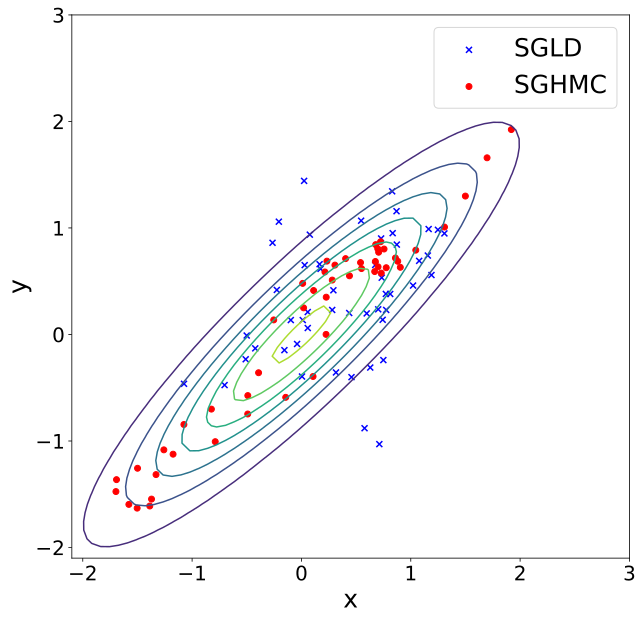
\includegraphics[width=.95\linewidth]{parts/Images/fig3b.pdf}
\caption{First 50 samples of SGHMC and SGLD}
\label{fig:b}
\end{subfigure}
\caption{Contrasting sampling of a bivariate Gaussian with correlation using SGHMC versus SGLD.}
\label{fig:demo}
\end{figure}

At last, to see more intuitively about the distributions of samples from SGHMC and SGLD, we reproduce Fig. 3(b) in original paper related to Fig. 3(b) here by showing the first 50 samples generated by the two samplers. We can conclude that SGLD's random-walk behaviour makes it perform worse to explore the tails of the distribution. However, SGHMC instead can drive the sampler to move along the distribution contours all the way around.

\subsection{Bayesian Neural Networks for Classification}
For the Bayesian neural network (BNN) MNIST classification we actually used the reparameterisation of SGHMC described in the section ``Connection to SGD with Momentum'' of \cite{sghmc}. The SGHMC algorithm is reframed in terms of learning rate and momentum decay, and simulates the following dynamics instead:
$$\begin{cases}
\nabla \theta = v\\
\nabla v = - \eta \nabla \wt{U}(\theta) - \alpha v + \mathcal{N}(0, 2(\alpha - \wh{\beta}) \eta)
\end{cases}
$$
where $\eta = \epsilon^2 M^{-1}, \alpha = \epsilon M^{-1}C, \wh{\beta} = \eta M^{-1}\wh{B}$. In all our experiments in this section we set the mass matrix $M $ to the identity, and the noise model $\wh{\beta} = \wh{B} = 0$. Other than the architecture of the BNN there are now only 3 hyperparameters for SGHMC, the learning rate $\eta$, the momentum decay $\alpha$ and the batch size $|\wt{\D}|$, in all our experiments we fixed $|\wt{\D}| = 500$ which follows from \cite{sghmc}.

To build on top of the work in \cite{sghmc} we implemented learning rate annealing for SGLD and following \cite{sgld} we weighted the samples by the learning rate as follows:
$$\mathbb{E}[f(\theta)] \approx \frac{\sum^T_{t=1} \epsilon_t f(\theta_t)}{\sum^T_{t=1} \epsilon_t}$$
Although since $f$ is a classifier we can ignore the denominator. Our BNN followed the same architecture as in \cite{sghmc}, that is one linear with 100 hidden units followed by ReLU activation followed by another linear layer and a log softmax for multi-class classification. The weights and biases for both linear layers are sampled from univariate standard normal distributions, but the Pyro method \texttt{to\_event()} declares dependence between the parameters. 

Our implementations of SGD and SGD with momentum are meant to be used directly with Pyro, and so Gaussian priors on the weights and biases is equivalent to L2 regularization in the non-Bayesian paradigm. We experimented with regularization strengths of $\lambda \in \{0.1, 1.0, 10.0\}$ and found $\lambda = 1.0$ to be the most effective. Additionally we implemented weight decay for both SGD and SGD with momentum but found that this didn't improve anything in this setting.

For the momentum based algorithms, SGHMC and SGD with momentum, we tried $\eta \in \{1.0, 2.0, 4.0, 8.0 \} \times 10^{-6}$, and $\alpha \in \{0.1, 0.01, 0.001 \}$. For SGHMC the best configuration was $\eta = 2.0\times 10^{-6}, \alpha=0.01$, and for SGD with momentum the best configuration was $\eta = 1.0\times 10^{-6}, \alpha=0.01$.

For SGLD and SGD, we tried $\eta \in \{1.0, 2.0, 4.0, 6.0\} \times 10^{-5}$, for SGLD we also tried learning rate annealing but it proved not to make much of a difference in this setting so we ignored it in the end. The best configuration for SGLD was $\eta = 4.0\times 10^{-5}$, and for SGD the best configuration was $\eta = 1.0\times 10^{-5}$.

For MNIST we ran each of the algorithms for 800 epochs with 50 warmup epochs. For the sampling algorithms we do Bayesian averaging over all the sampled parameterisations of the BNN after warmup as is described in Section II of \cite{hands-on-bnn} and report the test error. For the optimization algorithms we take most recent sample / set of parameters as a point estimate and report the test error.  Figure \ref{fig:MNIST} presents our results.

\begin{figure}[h!]
\centering
\includegraphics[width=100mm]{parts/Images/MNIST.png}
\caption{Reproducing the MNIST classification experiment from \cite{sghmc}; SGHMC ($\eta = 2.0\times 10^{-6}, \alpha=0.01, \texttt{resample\_n} =0$ ), SGLD ($\eta = 4.0\times 10^{-5}$), SGD ($\eta = 1.0\times 10^{-5}$), SGD with momentum ($\eta = 1.0\times 10^{-6}, \alpha=0.01$)}
\label{fig:MNIST}
\end{figure}
The results we get from MNIST classification align very closely with those in \cite{sghmc} and so we come to the same conclusion; the need for scalable and efficient Bayesian inference algorithms. The key benefit of BNNs is that we are not overconfident on out-of-distribution examples, Figure \ref{fig:B} illustrates that we still maintain this property when using SGHMC to approximately sample from the posterior distribution. We additionally conducted a brief comparison between Variational Inference (VI) and SGHMC in this setting, Figure \ref{fig:VI} outlines our findings.
\begin{figure}[h!]
\centering
\begin{subfigure}{.5\textwidth}
  \centering
  \includegraphics[width=.95\linewidth]{parts/Images/B.png}
  \caption{Uncertainty in out-of-distribution examples}
  \label{fig:B}
\end{subfigure}%
\begin{subfigure}{.5\textwidth}
  \centering
  \includegraphics[width=.95\linewidth]{parts/Images/VI_SGHMC.png}
  \caption{VI and SGHMC on MNIST}
  \label{fig:VI}
\end{subfigure}
\caption{{\bf Left} (a) illustrates that we get uncertainty estimates on out-of-distribution examples. {\bf Right} (b) compares VI (Renyi ELBO, $\alpha = 0.01$, \texttt{num\_particles} $= 2$) and SGHMC ($\eta = 2.0\times 10^{-6}, \alpha=0.01, \texttt{resample\_n} =0$) on MNIST. For VI we draw 80000 samples from the variational posterior $q_{\phi}$ and report the test error by Bayesian averaging. For SGHMC we do the same, except we are approximately sampling from the true posterior $p(\theta \: | D \:)$.}
\label{fig:demo}
\end{figure}
The initial results suggest that SGHMC performs better than VI in this setting, although this is not the full picture. Once VI fits the variational posterior distribution $q_{\phi}$ as closely as possible to the true posterior it takes only hundreds of samples to characterise $q_{\phi}$, whereas SGHMC requires several more samples to characterise the true posterior. In practice storing thousands of parameterisations of the same NN is very costly and so this is probably why VI is a more popular choice for Bayesian inference. 

We conclude this section by demonstrating our algorithms can be applied to other datasets and more complicated models, Figure \ref{fig:fashionMNIST} presents the results of running the same BNN architecture on FashionMNIST, and Figure \ref{fig:CIFAR10} demonstrates that our implementation of SGHMC can be used with convolutional neural networks (CNNs).
\begin{figure}[h!]
\centering
\begin{subfigure}{.5\textwidth}
  \centering
  \includegraphics[width=.95\linewidth]{parts/Images/fashion-mnist.png}
  \caption{Experiment on FashionMNIST}
  \label{fig:fashionMNIST}
\end{subfigure}%
\begin{subfigure}{.5\textwidth}
  \centering
  \includegraphics[width=.95\linewidth]{parts/Images/CIFAR10.png}
  \caption{Convolutional BNN on CIFAR10}
  \label{fig:CIFAR10}
\end{subfigure}
\caption{{\bf Left} (a) FashionMNIST classification; SGHMC ($\eta = 1.0\times 10^{-6}, \alpha=0.01, \texttt{resample\_n} =0$ ), SGLD ($\eta = 1.0\times 10^{-5}$), SGD ($\eta = 1.0\times 10^{-5}$), SGD with momentum ($\eta = 1.0\times 10^{-6}, \alpha=0.01$); \texttt{warmup\_epochs} $= 100$. {\bf Right} (b) Convolutional BNN with 2 convolutional layers, batch norm, max pooling and tanh activations followed by two Bayesian linear layers with tanh activation;  SGHMC ($\eta = 1.0\times 10^{-6}, \alpha=0.01, \texttt{resample\_n} =0$ ) ; \texttt{warmup\_epochs} $= 150$.}
\label{fig:other-datasets}
\end{figure}